% ============================================================

\begin{frame}{Candidate Supply Does Not Move, in Either Office}
\hypertarget{src:candidates}{}
\small
Litigation could thin the field as a \negt{barrier}, since suits are costly to mount and defend, or open it as a weapon, since a credible threat of challenge can deter a front-runner from standing. The sign is therefore ambiguous \emph{a priori}. Entry is also an anticipation margin: candidacies register at the August deadline \ns{(Lei 9.504, art.~11)}, before most suits resolve. Neither force shows up in the mayoral field or in the size of the council field.
\smallskip
\begin{center}
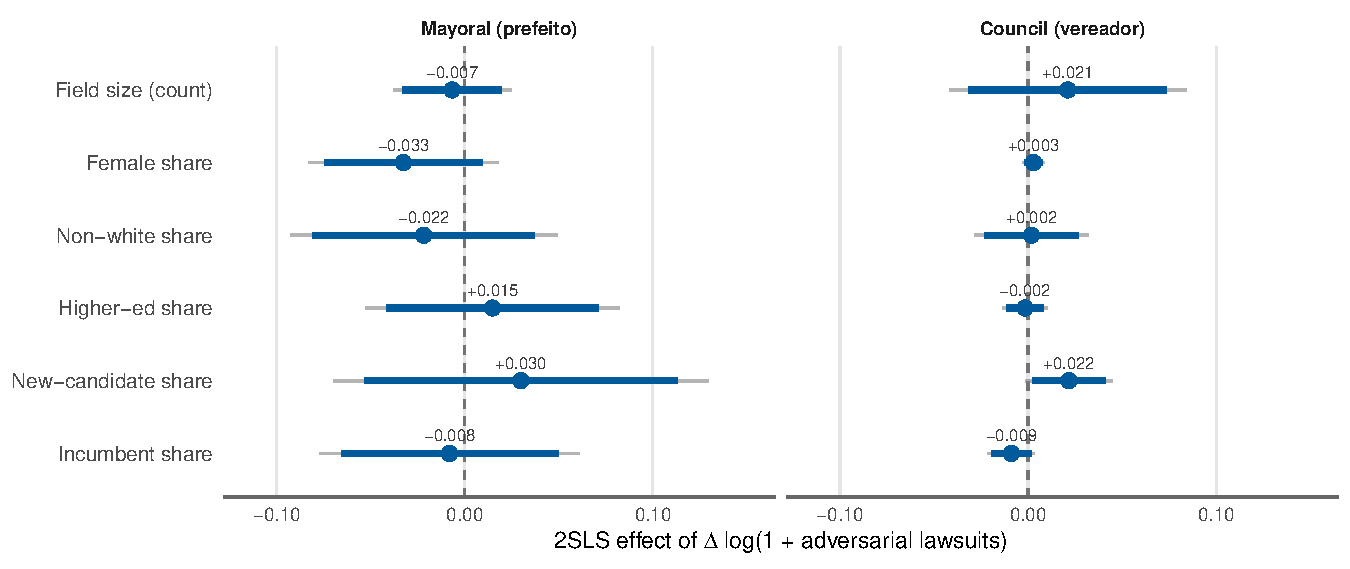
\includegraphics[width=\linewidth,height=0.44\textheight,keepaspectratio]{../figures/candidate_supply_coefplot.pdf}
\end{center}
\smallskip
\takeaway{No plotted supply margin moves in either office: mayoral field size ($\CandExecCoef$, $p=\CandExecP$), its female ($\FemaleCandCoef$, $p=\FemaleCandP$), non-white, higher-ed, new-entrant and incumbent shares, and the council pool ($\LegCandCoef$, $p=\LegCandP$) all straddle zero. Mean age is flat in the mayoral field (\MayorAgeYr~yr); the council pool is younger (\CouncilAgeYr~yr, $p=\CouncilAgeP$), one of \CouncilNSig{} of \CouncilNOutcomes{} council outcomes that clear 5\%; no council multiplicity correction is computed. What reshapes the race is therefore voter behavior, not the composition of the field.}\hfill\hyperlink{app:compbinary}{\beamergotobutton{count table}}
\end{frame}
